\documentclass[a4paper,12pt]{article}
\author{David Lorenz}
\title{The Boot Process on Microcontroller Systems}
\date{2023-04-09}

\usepackage[hidelinks]{hyperref}
\newcommand{\listingautorefname}{Listing}
\renewcommand{\subsectionautorefname}{Section}
\renewcommand{\subsubsectionautorefname}{Section}
\newcommand{\secref}[1]{\autoref{#1} \nameref{#1}}
\usepackage[printonlyused,withpage]{acronym}
\usepackage[utf8]{inputenc}
\usepackage{array}
\usepackage[title]{appendix}
\usepackage{booktabs}
\usepackage[
  backend=biber,
  style=numeric,
  sorting=none
]{biblatex}
\addbibresource{lorvEVA1.bib}
\DefineBibliographyStrings{american}{%
  urlseen = {url seen},
  and=\&,
  in=in
}
\usepackage{float}
\usepackage{svg}
\usepackage[bottom]{footmisc}
\usepackage{caption}
\usepackage{minted}
\usemintedstyle{solarized-light}
\definecolor{bg}{rgb}{0.95,0.95,095}
\setminted{
  linenos=true,
  autogobble,
  tabsize=4,
  breaklines,
  bgcolor=bg
}

\newcommand{\inlinec}[1]{\mintinline[bgcolor=bg]{c}{#1}}
\newcommand{\inlinebash}[1]{\mintinline[bgcolor=bg]{bash}{#1}}
\newenvironment{code}{\captionsetup{type=listing}}{}

\begin{document}
\maketitle
\thispagestyle{empty}
\newpage
\tableofcontents
\newpage

\section{Introduction}\label{sec:introduction}
On modern \ac{MCU} systems, the boot process is often neglected by application developers. The manufacturers provide the boot code with their \ac{SDK} and \ac{IDE}. Therefore application developers nowadays do not need to write this code themselves. In this document, I want to describe the different stages an \ac{MCU} runs through, from power-on or reset until the call of the main function. The ambition of this work is to show the absolute minimum number of steps an \ac{MCU} must perform in order to execute an application. Therefore, only bare-metal applications written in the C language, without the use of bootloader software, are covered. The level of detail in this document should be adequate to give other developers a good understanding of the boot process and a deepened knowledge of the systems they work with, without being overwhelming. This work is directed at other embedded application developers who have not yet looked into the boot process of their target micro-controllers and seek a better understanding of their target systems.
\par Some parts of the boot process are architecture- or implementation-specific and will vary on different \ac{MCU}s. To illustrate the key points in the boot process, the whole startup code as well as a custom linker script was written for an nRF52840 micro-controller from Nordic Semiconductors \cite{nrf52840Specification}. The example \ac{MCU} implements the ARMv7-M architecture. The goal of this work is to demonstrate the general key points of the boot process, but on a specific, real-world application. Most of the concepts are generally applicable, but beware, that the real-world example is based on a specific architecture and hardware implementation. The author aims to point out which aspects are specific to the example \ac{MCU} and which are universal. Both hard- and software aspects are explained. The major part lies in software and therefore needs more detailed documentation. It is crucial to have detailed knowledge of how the embedded software is built, in order to grasp all the key points of the boot code. Thus, the C build process is also covered in the software section.
\newpage

\section{Hardware}\label{sec:hardware}
Depending on the hardware in question, the hardware aspects of the boot process might vary, especially if the \ac{MCU} features a large variety of hardware peripherals. Two tasks have to be completed by every system before any code can be run. After a power cycle the \ac{MCU} has to wait for the supply voltage to stabilize and for the main oscillator to generate a stable sine wave for the internal clock generation \cite{microchip2023}. The \ac{OST} is used to guarantee that the signal from the oscillator is stable enough for the internal clock generation. \autoref{fig:ost} illustrates how the \ac{OST} works. After the output signal of the oscillator reaches a certain threshold, denoted as V\textsubscript{IH} and V\textsubscript{IL}, the timer waits a certain number of cycles before the internal clock is generated. In this case, the number of wait cycles is 1024. After the supply voltage is stable and the clock generation has started, the processor can start executing instructions. From this point on, the boot process is all software. The software will further initialize hardware it needs, but the supply voltage stabilization and the oscillator startup timer are the only parts that are completely in hardware.

\begin{figure}[H]
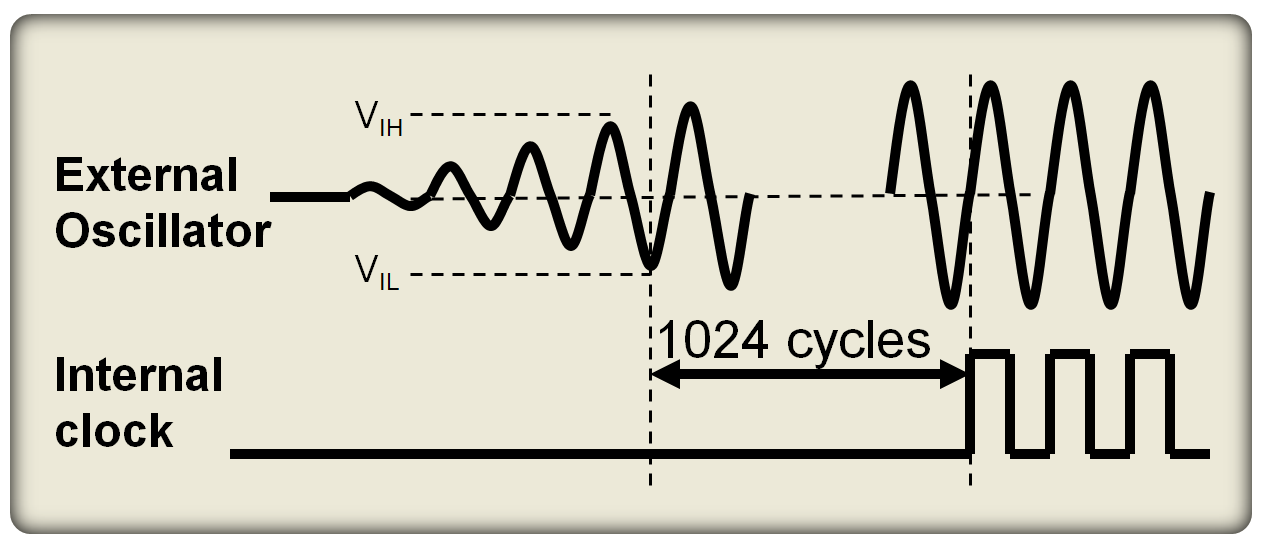
\includegraphics[scale=0.45]{graphics/ost.eps}
\centering{}
\caption{Oscillator Startup Timer \cite{microchip2023}}
\label{fig:ost}
\end{figure}
\newpage

\section{Software}\label{sec:minSoft}
In this chapter, we look at the code which is run before the main function of the application is called. Some of which is shipped with the chip and lies in \ac{ROM}. Other parts can be modified, but are usually provided by the manufacturer. We analyze the bare minimum of code that is needed to run an application on an \ac{MCU}. To understand the boot code, one needs to understand how software is built, therefore the relevant aspects of compilation and linking of software written in C is covered as well. To explain what happens in the boot process, the author wrote a minimal software project including a main function which toggles a \ac{LED}, a startup script and a linker script, for the nRF52840 development board form Nordic Semiconductors. The code we use in this section is based on the blog series "From zero to main()" by Francois Baldassari \cite{Interrupt}, but was adapted to work on the nRF52840 board and reduced to contain as little code as possible to get a working software. The full code can be found in \cite{lorv_eva1} to reproduce the results.

\subsection{Boot Code in \ac{ROM}}\label{sec:bootRom}
The first code that runs on an MCU is located in the so called boot \ac{ROM} and must be provided by the silicon manufacturer with the chip. The boot code depends on the architecture of the \ac{MCU} and on the hardware features it provides. ARM provides pseudo code for the boot code in the technical reference manual for each specific architecture that must be implemented by the silicon manufacturer. We will have a look at two different implementations and compare them in order to see, what kind of hardware features create differences in the boot code. The first one will be the ARMv6-M architecture with its implementations Cortex-M0, Cortex-M0+ and Cortex-M1. The second one is the ARMv7-M, which is the architecture for the Cortex-M3, Cortex-M4 and the Cortex-M7. The differences between the processors can be found in the Cortex-M comparison table \cite{ArmDevGuideCortexMCompTable}. \autoref{lst:armv6_boot} shows the pseudo code for the ARMv6-M architecture from the reference manual.

\begin{listing}[H]
  \inputminted{c}{code/armv6_reset_pseudo.txt}
  \caption{ARMv6-M boot \ac{ROM} pseudo code \cite{ARMv6-MRefManual}}
  \label{lst:armv6_boot}
\end{listing}

In short, what we see in the boot code, is that the core and special purpose registers of the \ac{MCU} are initialized. All events and exceptions are cleared. The stack pointer is initialized and then the second entry of the vector table, which is the reset handler, is loaded. The vector table contains the initial value of the stack pointer at reset and the entry point addresses of all the exception handlers, of which the reset handler is the first \cite{ARMv6-MRefManual}. 
\par Looking at the boot code in more detail, we see on line two that the \ac{VTOR} is set to zero. The vector table normally resides at address 0x00000000, but it can be relocated to a different location in memory. There are many reasons to relocate the vector table, which are out of scope of this work. If a relocation of the vector table is required, the new address must be stored in the \ac{VTOR}. The 13 general purpose registers will have unknown values in them. This is not something that has to be implemented in code, the pseudo code just states that this will be the case after a reset. The implementation does not need to write specific values to the general purpose register. A variable pointing to the vector table is defined and set to the value contained in the \ac{VTOR}. The current execution mode is set to thread mode. The processor can run in thread mode, which is for normal execution, or in handler mode, which is for handling exceptions. For more information about the different processor modes, consult \cite{ARMv6-MRefManual} or \cite{ARMv7-MRefManual}. The value of the \ac{LR} is also unknown at reset. The \ac{LR} holds the return address needed when returning from a subroutine. The \ac{APSR} too is unknown after reset. The \ac{APSR} is written to by certain instructions to give information about their result. For example, if an integer overflow has occurred. Consult \cite{ARMv6-MRefManual} for more information. The \ac{IPSR}, which holds the number of the exception currently being handled, is set to zero. The \ac{PRIMASK} is also cleared. The \ac{PRIMASK} is a one bit register. If it set to one, the priority of the current execution is set to zero, which means all exceptions, except reset, \ac{NMI} and hard fault are prevented. There are two different stacks on this architecture. The main stack and the process stack. In handler mode always the main stack is used, when in thread mode, the user can decide to use the process stack. In the CONTROL register the current stack is set to main. Further the software execution mode is set to privileged in the CONTROL register. More detailed information on all the core registers can be found in \cite{ArmDevGuideCoreRegisters}. Next, all the \ac{SCS} registers are reset. More information on the \ac{SCS} registers in \cite{ArmDevGuideSCSRegs}. Further, all 512 exceptions and the event register are cleared. Then, we set the main stack pointer to the address provided at the start of the vector table. The last two bits are set to zero, because, according to the \ac{ATPCS}, the stack must lay on an eight byte boundary \cite{ArmDevGuideAlignment}. The process stack pointer is unknown at this point, only that the two least significant bits must be zero, again to comply with the eight byte boundary specification. Finally, the address of the reset handler is loaded from the second position of the vector table, which is were the execution of the boot code ends and the execution of the first part of the user code starts.
\newpage Now let us have a look at the boot code of the ARMv7-M architecture and see where it differs from the one of ARMv6-M. We see in \autoref{lst:armv7_boot} that the boot code of the ARMv7-M is a bit more complex, but the differences are not that prominent. In addition to the \ac{PRIMASK} register, ARMv7-M offers the BASEPRI and FAULTMASK registers that must be cleared at reset. The priority of the current execution can be set to a custom value with the BASEPRI register. All exceptions lower than the value in the PRIMASK register are disabled. Similar to PRIMASK, setting the one bit register FAULTMASK to one, raises the priority level of the current execution to a fixed value. In this case to the level of a hard fault which is -1. This means if FAULTMASK is set, only a reset or a \ac{NMI} can preempt the current execution. The BASEPRI register sets the priority level of the current execution to a custom value. ARMv7-M offers an optional \ac{FPU}. On line seven of \autoref{lst:armv7_boot} is a check if a \ac{FPU} is present and if so, it is initialized. For a more detailed description of the registers concerning the \ac{FPU} consult the reference manual \cite{ARMv7-MRefManual}. The next difference we see is on line 36 where \inlinec{ClearExclusiveLocal()} is called. ARMv7-M offers instructions for atomic memory access, which ARMv6-M does not. The \inlinec{ClearExclusiveLocal()} function clears the local record for the atomic operation in the exclusive monitor. More information about the atomic instructions and the exclusive monitor can be found in \cite{ARMv7-MRefManual}. Setting the address of the vector table has a small difference too. On ARMv7-M only the bits 31 to 7 of the \ac{VTOR} are used and bits 6 to 0 are reserved, while on ARMv6-M the full 32 bit register is used. ARMv7-M has one more special purpose register which is not present in version 6, the \ac{EPSR}. The \ac{EPSR} contains, among others, the t-bit, which has to be set to 1 to indicate that the processor is executing thumb instructions. The ARMv6-M and ARMv7-M both only support thumb instructions so this is mandatory. The rest of the \ac{EPSR} is set to zero. Again consult \cite{ARMv7-MRefManual} for more detailed information.

\begin{code}
  \inputminted{c}{code/armv7_reset_pseudo.txt}
  \caption{ARMv7-M pseudo boot code \cite{ARMv7-MRefManual}}
  \vspace{1.5em}
  \label{lst:armv7_boot}
\end{code}

In general the more features a processor offers, the more complex the boot \ac{ROM} code will be. ARMv7-M contains more core- and special purpose registers since it offers a larger number of features. The presence of a co-processor, in this case a \ac{FPU} also leads to more boot code, since that additional core must be initialized as well. On different architectures, one would find different boot code, but the principle would stay the same. Bring the registers to their initial state, initialize co-processors, load the stack pointer and once the processor is in the desired state, branch out to the reset handler.

\subsection{C Software Build Process}\label{sec:buildProcess}
We have seen in the \nameref{sec:bootRom} section that at the end of the boot code the initial stack pointer is loaded into the SP register from address 0x00000000 and the initial program counter from address 0x00000004. Then the reset handler is executed. In order to understand where the addresses come from and how the right values end up at these memory locations, we need to understand how C software is built. Especially the linking phase is of interest to explain what happens during boot, but for the sake of completeness, the whole build is briefly explained here.\par
\autoref{fig:Cbuild} shows a flow diagram of how compiler toolchain build an executable from C code. The build process consists of several phases.

\begin{figure}[H]
  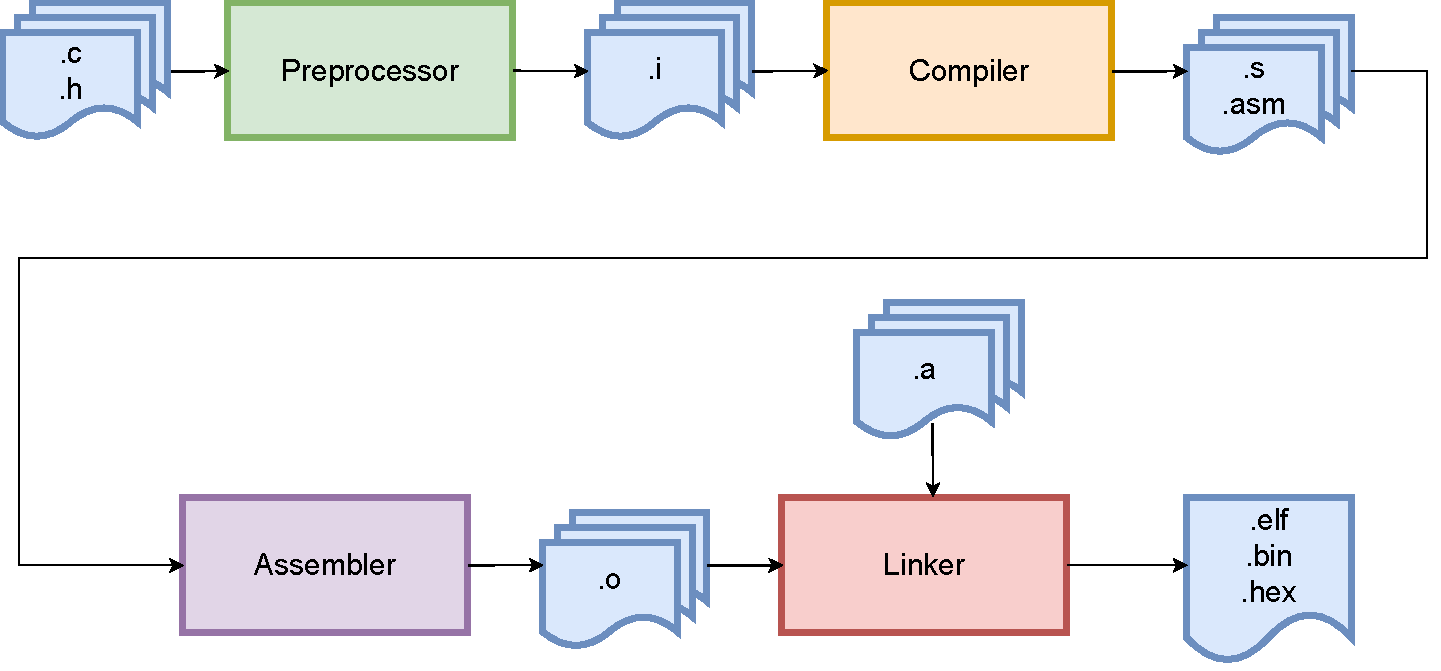
\includegraphics[scale=0.55]{graphics/CBuildProcess.pdf}
  \centering{}
  \caption{C build process flow}
\label{fig:Cbuild}
\end{figure}

To explain some of the concepts of the build process we will examine a code example during different stages of the build process. Have a look at the code in \autoref{lst:buildCode}. On lines three to six we declare or initialize \footnote{Declaration: Creation of a symbol; Definition: Memory is allocated for the symbol; Initialization: A value is written to the memory location of the symbol.} a number of variables with different attributes. We will see later how those variables end up in different sections of our memory and have different scopes because of their attributes.

\begin{listing}
  \inputminted{c}{code/build_example.c}
  \caption{Example code for build process}
  \label{lst:buildCode}
\end{listing}

If not specified otherwise, the compiler will produce three memory sections and assign every label to one of them. Of course, one is free to define any number of sections. More complex software will most certainly have more sections than the ones described here, but these are necessary for even the simplest software. The sections are:

\begin{itemize}
  \item data-section - All global and local variables which have been assigned a specific value are located here.
  \item bss-section - All global and local variables which are not initialized with a value go in the bss-section. This section needs to be initialized to zero before the execution of the program starts.
  \item text-section - In the text-section reside the functions of the program.
\end{itemize}

We will have a detailed look at these sections in \secref{sec:linkerScript}, where we will describe how they are built in memory.

\paragraph{Preprocessor}\label{sec:preProc}
The preprocessor takes the source code, in other words all the .c and .h files in a project, as input and produces .i files as output. The preprocessor reacts to preprocessor directives which start with the \#-character like the \mintinline{c}{#include} directive. With preprocessor directives one can include or exclude code-section depending on \mintinline{c}{#define} statements, like in the example in \autoref{lst:preproc}. The function \inlinec{foo} is only present in the output code of the preprocessor, if \inlinec{USE_FOO} is defined. Otherwise the code for \inlinec{foo} will be stripped out of the code. The preprocessor is also responsible for expanding all C-macros to actual code and removing all comments. For a detailed description of GCC's preprocessor functions consult its manual \cite{GccGNUOnlneDocsCPreProc}.

\begin{listing}[H]
\inputminted{c}{code/preproc.c}
  \centering
  \caption{C preprocessor directive example}
  \label{lst:preproc}
\end{listing}

\paragraph{Compiler}\label{sec:compiler}
The compiler takes the .i files from the preprocessor and generates assembly instructions in .s or .asm files. The assembly instructions are hardware dependent, therefore the compiler needs to know which target hardware the code is compiled for. The compilation phase includes a hardware-independent frontend and a hardware-dependent backend. In general, the frontend carries out code analysis while the backend performs code synthesis. In more detail the frontend conducts:

\begin{itemize}
  \item Lexical Analysis - Tokenization of keywords, identifiers, operators and literals
  \item Syntax Analysis - Scans the tokens to ensure C language compliance
  \item Semantic Analysis - Type checking, label checking and flow control checking
\end{itemize}

The compiler backend is responsible for:

\begin{itemize}
  \item Code generation - Translation of the frontend output to actual assembly instructions
  \item Optimization - Optimize the generated code according to settings
\end{itemize}

Along the assembly code, the compiler also generates the symbol table, which is needed during analysis and synthesis. Symbols in general are references to variable names and function names. Symbols are used in every step of the build process. The symbol table stores the names, the types and the scope of all symbols on an object file level \cite{EmbeddedSecurity}\cite{TutorialsPoint}.\par

If we want to examine the assembly code the compiler produces for our example, we can use the following command:\newline

\inlinebash{arm-none-eabi-gcc -S -o build_example.s build_example.c}\newline

The whole assembly code generated by the compiler for our example code from \autoref{lst:buildCode} can be found in Appendix A1 in \autoref{lst:buildAssembly}.

\paragraph{Assembler}\label{sec:assembler}
The next stage in the build process is assembly. Here, the assembly code is translated to the equivalent opcodes of the target hardware. While the assembly code is, although cumbersome, still human readable, the opcode is in binary form and no longer readable by humans. It is placed in object files with the .o file ending. The symbols in the object files do not contain the symbols full addresses, but only the section in which they belong and their offset from the start of the section.

We can build the object file of our example code with the following command:\newline

\inlinebash{arm-none-eabi-gcc -c -o build_example.o build_example.c}\newline

We can now inspect the symbols in our object file to see what happened to our variables and functions with \inlinebash{arm-none-eabi-nm}. The \inlinebash{nm} command shows us the symbol names, their corresponding addresses, in which section they are and with what scope. If we use the \inlinebash{-S} option, it also prints the size. The output of the command above is shown in \autoref{lst:nmOutput}.

\begin{listing}
  \inputminted{text}{code/build_example_nm.txt}
  \caption{Output of \inlinebash{nm} command}
  \label{lst:nmOutput}
\end{listing}

The first column of the output is for the address of the symbol. At this point the addresses are not known so we only see the offset of the symbol from the start of the memory section it lies in. The actual addresses will be assigned by the linker in the next stage of the build process. Three of the symbols have an offset of zero, because they are at the beginning of their corresponding section. In the second column, we see the size of the symbol. The third column describes the type. \autoref{tbl:nmSymbolType} shows a description of the symbol types. In general an uppercase letter in the type field means global scope and a lower case letter local scope. For more detailed information check the manpage of the \inlinebash{nm}-command.

\begin{table}[H]
\begin{tabular}{@{}llr@{}} \toprule
Symbol & Description \\ \midrule
U & Undefined \\
B/b & bss-section \\
D/d & data-section \\
T/t & text-section\\ \bottomrule
\end{tabular}
\centering
\caption{\inlinebash{nm} command symbol types}
\label{tbl:nmSymbolType}
\end{table}

We see in \autoref{lst:nmOutput} that \inlinec{extern volatile int global_var} and\newline \inlinec{static int local_var_data} both are in the data-section of the memory. This makes sense, since they both are initialized to a specific value. Since \inlinec{int global_var} is of type \inlinec{int}, and an \inlinec{int} takes up 4 byte of memory, on gcc compiler, which we used to compile this code, we see that the offset of \inlinec{local_var_data} from the start of its section makes perfect sense as well. Our functions both go to the text-section and \inlinec{local_var_bss} resides in the bss-section. So far, everything is as one would expect from looking at the example code in \autoref{lst:buildCode}. The two undefined symbols do not contain an address offset, because they are not defined in this file. \inlinec{extern_var} is only declared in the code and we tell the compiler with the \inlinec{extern} keyword, that the definition of this variable is elsewhere. Remember that there is only one file in our example code, this means there is no definition of \inlinec{extern_var}. The compiler is completely happy with this, since it is not its job to assign an actual address to this symbol. The linker on the other hand, whose job it is to assign said address, will not be happy, unless we link this code against another file, which holds the definition of this variable. The same goes for the \inlinec{printf}-function, but here we are in a better position. Although the included stdout.h file only holds the prototype of the function, which implies the \inlinec{extern} keyword, the linker will find the implementation of the function if we link against the standard library, which we do. Therefore, the linker is able to resolve this undefined reference.\newpage

\paragraph{Linker}\label{sec:linker}
Linking is the final step in the build process. It takes all the assembled object files and object files of external libraries and produces a single file, which is the executable. The object files each have their own data, bss and text sections. The linker combines these sections in the executable so that each section only appears once. This process is called merge and relocation \cite{EmbeddedSecurity}. As mentioned above, the linker is responsible of resolving all the undefined symbols in the symbol table. If this is not possible the linker will throw an undefined reference error. Additionally, the linker assigns the actual addresses to all the symbols. In order to do this, the linker uses the so called linker script, where we define the memory layout of the target \ac{MCU} and where in memory we want our sections to be located. The linker script is explained in more detail in \secref{sec:linkerScript}, with a real example of a minimal script for our example hardware, the nRF52840 development kit from Nordic Semiconductors.

\subsection{Linker Scripts}\label{sec:linkerScript}
In this section, we will construct a small custom linker script, which will then be used to link our minimal software. We will only discuss the elements needed for almost every software and not go into details about the command language of the linker. For more details about the language, consult the Command Language section of the GNU Linker documentation \cite{GNUBInutils}. The first thing we need to specify in the linker script is the memory layout of our target hardware. The nRF52840 contains 1024kB of flash memory and 256kB of \ac{RAM} which use the base addresses 0x00000000 and 0x20000000, respectively \cite{nrf52840Specification}. With this information, we can construct the memory layout in the linker script as shown in \autoref{lst:LinkMem}. The \inlinebash{ORIGIN} keyword specifies the base address and the \inlinebash{LENGTH} the size of the region. The \inlinebash{rx} respectively \inlinebash{rxw} attributes in the braces describe the properties of the memory region. Those attributes do not set the properties but only describe them \cite{GNUBInutils}.

\begin{listing}[H]
  \inputminted[firstline=1, lastline=5]{bash}{code/nrf52840_report_ld.ld}
  \caption{Linker script memory layout}
  \label{lst:LinkMem}
\end{listing}

Next we need to define our sections, beginning on line 7 of \autoref{lst:LinkText}, and tell the linker where to put them. We start with the text-section. On line 9, we define the text-section of the output file, which is the executable. Inside the curly braces, we relocate the symbols from the object files to the text-section of the executable. The syntax to relocate a symbol from an input file to a section in the output file is \inlinebash{<filename>(<section><symbol>)}. On line 12 we combine all the text sections from all the input files to the text-section of the output file. We use the *-wildcard for the filename to tell the linker to perform this action on every object file and use a wildcard at the end to include every symbol from the text-section, of that particular file. On line 11 we place the vector table at the beginning of our text-section. We will see where it comes from in \secref{sec:startupScipt}. The \inlinebash{KEEP} keyword is used so the vector table is kept in the text-section, even though no symbols inside it are ever referenced in the code \cite{OSdevWiki}. On line 13 we insert a new symbol into the text section. The \inlinebash{.} character denotes the address where the linker currently is. So the symbol we insert is called \inlinebash{_etext} and it lies at the end of the text-section. By referencing this symbol in the code, we get the address where the text-section ends. We will see why this is useful in \secref{sec:startupScipt}. On line 14 we tell the linker, that the text-section resides in the \ac{ROM} area of our memory.

\begin{listing}
  \inputminted[firstline=7, lastline=14]{bash}{code/nrf52840_report_ld.ld}
  \caption{Text-section in the linker script}
  \label{lst:LinkText}
\end{listing}

The next section to be defined is the bss-section as shown in \autoref{lst:LinkBss}. As explained in \secref{sec:buildProcess}, all uninitialized static variables are placed here. With the \inlinebash{NOLOAD} keyword on line 16 we specify that there are no values to be loaded in this section, since all these variables must be initialized to zero, by the software. We will see how this is done in \secref{sec:startupScipt}. We have two input sections from our object files, the bss-section which contain all the uninitialized local variables and the COMMON-section, which includes all the uninitialized global variables. Analog to the \inlinebash{_etxt} symbol in the text-section, we insert new symbols to mark the beginning and end of the bss-section on lines 18 respectively 21. On line 22 we specify the bss-section to be in \ac{RAM}.

\begin{listing}
  \inputminted[firstline=16, lastline=22]{bash}{code/nrf52840_report_ld.ld}
  \caption{bss-section in the linker script}
  \label{lst:LinkBss}
\end{listing}

As previously explained, the data-section holds all the static variables, which are initialized to a non-zero value. The data-section follows the same principle as the other two but has one peculiarity. The data-section lies in \ac{RAM} during execution, but the initial values of the variables must also be stored in flash so that they are not lost on a reset. When the \ac{MCU} boots, the initial values must be copied from flash to ram. We will see where this memory transfer is done in \secref{sec:startupScipt}. On line 29 of \autoref{lst:LinkData}, we tell the linker that there are two different addresses for this section. The first one is the \ac{VMA}, where the variables are stored during program execution. The second one is the \ac{LMA} where the initial values of the variables are stored. With the \inlinebash{AT} attribute, we tell the linker that this sections \ac{LMA} is different from its \ac{VMA}.

\begin{listing}
  \inputminted[firstline=24, lastline=29]{bash}{code/nrf52840_report_ld.ld}
  \caption{data-section in the linker script}
  \label{lst:LinkData}
\end{listing}

The minimal software also needs a stack and therefore a stack-section must be defined in the linker script. The relevant code to initialize a stack-section is shown in \autoref{lst:LinkStack}. First, the size of the stack is defined on line 31. Like the bss-section, the stack-section does not need any values loaded into it. That is why this section has the \inlinebash{NOLOAD} attribute as well. The \ac{ATPCS} specifies that the stack needs to be eight byte aligned \cite{ArmDevGuideAlignment}, so on lines 36 and 39 this alignment is implemented. At the end of the linker script we align to a four byte boundary and add a symbol to mark the end of the used memory. The full code of the linker script can be found in \cite{lorv_eva1}.

\begin{listing}
  \inputminted[firstline=31, lastline=45]{bash}{code/nrf52840_report_ld.ld}
  \caption{data-section in the linker script}
  \label{lst:LinkStack}
\end{listing}

\subsection{Startup Script}\label{sec:startupScipt}
As seen in \secref{sec:bootRom}, at the end of the boot code the second entry in the vector table is called. From \secref{sec:bootRom} we also know, that the second entry in the vector table must be the reset handler. The startup script is responsible for putting the vector table at the right location in memory. Further the code of the exception handlers is also located in the startup script. Normally, the startup script is provided for application developers by the \ac{MCU} manufacturer. It is usually written in assembly \cite{Interrupt}. See \cite{nrfxDriverCollection} for the one that Nordic Semiconductor provides for the nRF52 series. In order to explain what takes effect in the startup script, we will write one ourselves in C. The startup script is responsible for bringing the processor to a state from which the main application can be executed, and actually call the main function. In our minimal software example, we must implement the mandatory exception handler functions in the vector table, which are:

\begin{itemize}
  \item reset handler
  \item NMI handler
  \item hard fault handler
\end{itemize}

Further we need to populate the vector table with the pointers to the handlers and the initial stack pointer. In the reset handler, we need to initialize the data- and bss-sections in \ac{RAM} and call the main function. \autoref{lst:strtDecl} shows all the declarations needed in the startup script. On lines four to ten, we see the symbols we defined in the linker script, declared as external variables. The linker will resolve those references for us. The values of those variables are of no use to us. We only want the location in memory of the start and end of our sections. So we only use their addresses in the code. On lines 13 to 15, we declare the exception handler functions. Note the forward declaration of the main function, which is needed since we must call main in the reset handler.

\begin{listing}
  \inputminted[firstline=3, lastline=18]{c}{../code/nrf52840-from-scratch/nrf52840_startup.c}
  \caption{Startup script declarations}
  \label{lst:strtDecl}
\end{listing}

\newpage
In \autoref{lst:strtVec} we see the declaration and definition of the vector table. We have a few interesting lines of code here which need some explanation. On line 29 we specify two variable attributes which apply to the \inlinec{vectors} array. The \inlinec{used} attribute is needed so the variable will not be optimized away by the compiler because it is never used \cite{ArmDeveloperDocCompSpecFeat}. The \inlinec{section} attribute is used to mark a new section in the code \cite{ArmDeveloperDocCompSpecFeat}. We have already seen this section in the linker script, where we tell the linker to relocate this section to the beginning of the text-section. On line 30 we declare an array named \inlinec{vectors}. The array contains pointers constants to functions which take no arguments and have no return value. On lines 31 to 36 we define the actual array. On line 32 we populate the first entry of the vector table, which is the initial stack pointer. We use the address of the \inlinec{_estack} variable we declared earlier. The \inlinec{_estack} variable is of type \inlinec{uint32_t}, therefore we must cast its address to the type of the exception handlers.

\begin{listing}
  \inputminted[firstline=29, lastline=36]{c}{../code/nrf52840-from-scratch/nrf52840_startup.c}
  \caption{Definition of the vector table}
  \label{lst:strtVec}
\end{listing}

Now we define the actual reset handler in \autoref{lst:strtReset}. First, we copy the initial values of the variables in the data-section from flash to \ac{RAM}. To achieve this we define a few pointers to the addresses from the symbols we inserted in the linker script. On line 45 we check if there even is a data-section to be copied, otherwise we skip the for loop which does the actual data transfer. Next, we initialize the bss-section to zero. In our example code, we then call the main function and insert an infinite loop in case the main function returns for some reason. In the startup script from Nordic Semiconductors there is an additional call to a system init function. In this function workarounds for hardware errors and other hardware initialization according to preprocessor flags is done. Since our goal was to implement the most basic start up code possible, we skip this further initialization. The main function of our example software only toggles one \ac{LED} by writing directly to registers and therefore we do not need the functionality implemented in the system init function. In a real-world application, it would be inadvisable to take this approach. For the \ac{NMI} handler and the hard fault handler, we only implement infinite loops. The full code can be found in \cite{lorv_eva1}. 

\begin{listing}[H]
  \inputminted[firstnumber=38]{c}{../code/nrf52840-from-scratch/reset_handler.c}
  \caption{Definition of the reset handler}
  \label{lst:strtReset}
\end{listing}

\newpage
\section{Conclusion and Outlook}
This work shows, that the parts of the boot code outside the \ac{ROM} can be implemented with relatively little effort. However it is not recommended to do this, except for educational purposes. The \ac{MCU} manufacturers provide the boot code for their processors and it should be used for many reasons.\par
All the stages of the boot process are covered and additional information is provided or referenced to present a full explanation for other developers to work with. During the formation of this document it became clear, that the build process of the software needs to be fully understood in order to understand the boot code completely, so one section is dedicated to the software build process.\par However in this work only the most trivial form of the boot process is covered. In future work more complex implementations like bootloader software, booting from external memory and the influences on the boot process of an \ac{OS} or \ac{RTOS} could be discussed. An other topic related to the boot process is security. How can a secure boot be guaranteed, so that only trusted software is executed on the \ac{MCU}?\newpage


\section*{List of Acronyms}
\begin{acronym}
  \acro{MCU}{Micro Controller Unit}
  \acro{SDK}{Software Development Kit}
  \acro{IDE}{Integrated Development Environment}
  \acro{SoC}{System on Chip}
  \acro{OST}{Oscillator Startup Timer}
  \acro{ROM}{Read-Only Memory}
  \acro{RAM}{Random Access Memory}
  \acro{LED}{Light Emitting Diode}
  \acro{ATPCS}{ARM-Thumb Procedure Call Standard}
  \acro{LR}{Link Register}
  \acro{APSR}{Application Program Status Register}
  \acro{IPSR}{Interrupt Program Status Register}
  \acro{PRIMASK}{Priority Mask Register}
  \acro{SCS}{System Control Space}
  \acro{VTOR}{Vector Table Offset Register}
  \acro{EPSR}{Execution Status Register}
  \acro{FPU}{Floating Point Unit}{}
  \acro{NMI}{None Maskable Interrupt}
  \acro{LMA}{Load Memory Address}
  \acro{VMA}{Virtual Memory Address}
  \acro{OS}{Operating System}
  \acro{RTOS}{Real Time Operating System}
\end{acronym}

\printbibliography

\begin{appendices}
\section{Code}
\subsection{Assembly code of the build example}\label{sec:AssmblCode}
\begin{code}
  \inputminted{ca65}{code/build_example.s}
  \caption{Assembly of the Build Example Code From \autoref{lst:buildCode}}
  \label{lst:buildAssembly}
\end{code}
\end{appendices}
\end{document}